\section{Introduction}\label{sec:intro}

The \emph{skew Schur polynomials} are a fundamental family of symmetric polynomials whose connection to representation theory was first studied by I.~Schur. This family is indexed by \emph{skew partitions} $\lambda / \mu$, where $\lambda = (\lambda_1 \geq \lambda_2 \geq \cdots \geq \lambda_n > 0)$ and $\mu = (\mu_1 \geq \mu_2 \geq \cdots \geq \mu_m > 0)$ are \emph{partitions} with $\mu \subseteq \lambda$ (that is, $m \leq n$ and $\mu_i \leq \lambda_i$ for $1\leq i \leq m$). The skew Schur polynomial of \emph{shape} $\lambda / \mu$ is the generating function
\begin{equation}
\label{eqn:skewpolydef}
s_{\lambda / \mu}(x_1,\ldots,x_n) = \sum_T x^{\eta(T)}, \qquad x^{\eta(T)}\coloneqq x_1^{\eta_1(T)}x_2^{\eta_2(T)}\cdots x_n^{\eta_n(T)},
\end{equation}
where the sum is over all semistandard tableaux $T$ of shape $\lambda / \mu$ with entries in $[n]$, and $\eta_i(T)$ is the number of entries in $T$ equal to $i$.

Though not immediately apparent from~\eqref{eqn:skewpolydef}, $s_{\lambda / \mu}(x_1,\ldots,x_n)$ is an element of $\Lambda_n$, the ring of symmetric polynomials in variables $x_1,\ldots,x_n$. For $\lambda = (\lambda_1, \lambda_2, \hdots ,\lambda_n )$, the \emph{length} of the partition is $\ell(\lambda) = n$. Defining $s_{\lambda}(x_1,\ldots,x_n) \coloneqq s_{\lambda / \emptyset}(x_1,\ldots,x_n)$ we recover the \emph{Schur polynomials}; the $s_{\lambda}(x_1,\ldots,x_n)$ with $\ell(\lambda) \leq n$ are a $\mathbb{Z}$-linear basis of $\Lambda_n$. This implies
\begin{equation}
\label{eqn:skewdecomp}
s_{\lambda / \mu}(x_1,\ldots,x_n) = \sum_\nu c_{\mu,\nu}^{\lambda} s_{\nu}(x_1,\ldots,x_n)
\end{equation}
where the sum is over partitions $\nu$ with $\ell(\nu) \leq n$ and the coefficients $c_{\mu,\nu}^{\lambda}$ are the celebrated Littlewood--Richardson coefficients. The expansion~\eqref{eqn:skewdecomp} is \emph{multiplicity-free} if $c_{\mu,\nu}^{\lambda} \in \{0,1\}$ for all $\nu$ with $\ell(\nu) \leq n$. A natural question is then: 
\[
\text{When is $s_{\lambda / \mu}(x_1,\ldots,x_n)$ multiplicity-free?}
\] 
Our Theorem~\ref{theorem:mainResult} gives a complete, non-recursive answer to this question.

\subsection{Multiplicity-free representation theory} Multiplicity questions, along the same line as the one posed above, have both representation theoretic and geometric import. The Schur polynomials are characters of the irreducible polynomial representations of $GL_n$ (and of $SL_n$, but we focus here on $GL_n$). Expressing a $GL_n$ representation character in the basis of Schur polynomials is equivalent to decomposing the representation into a sum of irreducible representations. 

Knowing that a representation is multiplicity-free has a number of applications (see, \eg the survey~\cite{H95}). Pivoting to a geometric perspective, a group action on a projective algebraic variety induces an action on its homogeneous coordinate ring. The representations that arise from this induced action can often illuminate the orbit structure of the group in the variety~\cite{AP14,MWZ01,P14,S03}. In~\cite{HL19}, the second author and V.~Lakshmibai classified \emph{spherical Schubert varieties} by showing that certain infinite sets of skew Schur polynomials always contain elements that are not multiplicity-free. 

Developing multiplicity-free criterion for important families of representations has seen considerable interest. In~\cite{S01}, the prototypical example, J.~Stembridge classified products of Schur functions that are multiplicity-free. In \emph{ibid.}, he extended this to a classification of the multiplicity-free products of Schur polynomials (equivalently multiplicity-free tensor products of irreducible $GL_n$ representations). The skew Schur functions whose coefficients are all equal to $1$ over an entire dominance order interval, and equal to $0$ otherwise, are characterized in~\cite{ACM19}. Other examples of multiplicity-free classifications include~\cite{FMS19,G10,TY10}. As the skew Schur polynomials are $GL_n$ characters of the skew Schur modules~\cite{FH91}, this paper represents our contribution to this body of work. 

\subsection{Main theorem} Altering definition~\eqref{eqn:skewpolydef} so that it becomes a sum over all semistandard tableaux of shape $\lambda / \mu$ yields the \emph{skew Schur function} $s_{\lambda / \mu}$. In~\cite{TY10}, H.~Thomas and A.~Yong classified multiplicity-free products of Schubert classes in the cohomology ring of the Grassmannian. As the authors note, this is equivalent to classifying multiplicity-free skew Schur functions (see also~\cite{G10}). 

Implicitly, $s_{\lambda / \mu}(x_1,\ldots,x_n)$ is a specialization of $s_{\lambda / \mu}$ that arises by setting $x_m=0$ for $m > n$. In particular, if $s_{\lambda / \mu}$ is multiplicity-free, then so is $s_{\lambda / \mu}(x_1,\ldots,x_n)$, but the converse does not hold. In this sense, our classification is a generalization of~\cite{TY10}, and we follow much of their terminology and notation.

 Our result relies on four reductions. The first is central to~\cite{TY10}. A partition $\lambda$ is visualized by its \emph{Young diagram}, also denoted $\lambda$; it is a collection of left justified boxes, with $\lambda_i$ boxes in row $i$. Analogously, given a skew partition $\lambda / \mu$, the \emph{skew (Young) diagram} $\lambda / \mu$ equals the Young diagram $\lambda$ with the leftmost $\mu_i$ boxes deleted in each row $i$.

\begin{exam}\label{ex:skewshape}
Let $\lambda = (5,4,1,1)$ and $\mu = (2,1,1)$. The Young diagrams $\lambda$, $\mu$ and the skew diagram $\lambda / \mu$ are listed below, left to right.
%\begin{center}
\[
\ytableausetup{boxsize=1em}
\begin{ytableau}
\; & \; & \; & \; & \; \\
\; & \; & \; & \; \\
\; \\
\; \\
\end{ytableau}
\qquad \qquad \qquad
\begin{ytableau}
\; & \; \\
\; \\
\; \\
\end{ytableau}
\qquad \qquad \qquad
\begin{ytableau}
\none & \none & \; & \; & \; \\
\none & \; & \; & \; \\
\none \\
\; \\
\end{ytableau}
\] %\end{center}
\end{exam}

If there is a box $B$ in row $r$ and column $c$ of the skew diagram $\lambda / \mu$ we will write $B = (r,c) \in \lambda / \mu$. Then $\colsf (B)=c$ and $\rowsf (B)=r$. For any set $S \subset [\lambda_1]$, we refer to column $k$ as an $S$-column if $k\in S$.
\begin{defi}
A skew partition is \emph{basic} if its skew diagram does not contain any empty rows or columns. The skew partition that arises from the deletion of all empty rows and columns of $\lambda / \mu$ is called the \emph{basic demolition} of the skew partition, and is denoted $(\lambda / \mu)^{\ba }$.
\end{defi}


Let $\CS_k(\lambda / \mu)=|\{r : (r,k) \in \lambda / \mu \}|$ be the number of boxes in the $k$-th column of $\lambda/\mu$. Define
\begin{equation}
\rho(\lambda / \mu) \coloneqq \max\{\CS_k(\lambda / \mu) : 1 \leq k \leq \lambda_1\}
\end{equation} 
to be the maximal number of boxes in any column of $\lambda/\mu$. In Example~\ref{ex:skewshape}, $\rho(\lambda/\mu) = 2$.

\begin{defi} \label{def:nsharpandnsharpdemo} A skew partition is $n$-\emph{sharp} if $\CS_k(\lambda / \mu) < n$ for all $k$. The $n$-\emph{sharp demolition} of a skew partition is equal to $\emptyset / \emptyset$ if there exists a $k$ such that $\CS _k(\lambda / \mu) > n$. Otherwise
it equals the skew partition that remains after deleting each column $k$ such that $\CS _k(\lambda / \mu) = n$. We denote the $n$-sharp demolition by $(\lambda / \mu)^{n\sharp}$.
\end{defi}

In Example~\ref{ex:skewshape}, if $n=2$, then $(\lambda/\mu)^{n\sharp}$ is
\[
\begin{minipage}[c]{20mm}
\ytableausetup{boxsize=1em}
\begin{ytableau}
\none & \none & \none & \none & \; \\
\none & \; & \none & \none \\
\none \\
\; \\
\end{ytableau}
\end{minipage}.
\]
If $n=1$, then $(\lambda/\mu)^{n\sharp} = \emptyset / \emptyset$.

When convenient, a partition will be presented as $(\lambda_1^{l_1},\lambda_2^{l_2},\ldots,\lambda_p^{l_p})$ where $\lambda_1\geq \cdots\geq \lambda_p$. This corresponds to the partition with the first $l_1$ entries equal to $\lambda_1$, the next $l_2$ entries equal to $\lambda_2$, and so on. The {\em number of parts} of $\lambda$ is $\np (\lambda) = p$. If $\np (\lambda)=1$, the partition is called a \emph{rectangle}. A partition $\lambda$ with $\np (\lambda)=2$ is called a \emph{fat hook}. 

For a skew partition $\lambda/\mu$ where $\lambda = (\lambda_1^{l_1},\lambda_2^{l_2},\ldots,\lambda_p^{l_p})$ and $\mu = (\mu_1^{k_1},\mu_2^{k_2},\ldots,\mu_q^{k_q})$, define $\tau(\lambda / \mu) = \sigma(\lambda/\mu) = 0$ if $\mu = \emptyset$ or $\lambda$ is a rectangle.
Otherwise, define
\begin{equation}
\tau(\lambda / \mu) = l_1 - \min(l_1,\ell(\mu))\text{ and }
\sigma(\lambda/\mu) = \lambda_p - \min(\mu_1, \lambda_p).
\end{equation}

\begin{defi} \label{def:tightandtightdemo} A basic skew partition $\lambda/\mu$ is \emph{tight} if $\tau(\lambda / \mu) = \sigma(\lambda/\mu) = 0$. The \emph{tight demolition} of $\lambda / \mu$ is 
\[
(\lambda / \mu)^{\ti } = (((\lambda_1-\sigma(\lambda/\mu))^{l_1 - \tau(\lambda / \mu)},(\lambda_2-\sigma(\lambda/\mu))^{l_2},\ldots,(\lambda_p-\sigma(\lambda/\mu))^{l_p}) / \mu)^\ba . 
\] 
Note that if $\tau(\lambda / \mu) = \sigma(\lambda/\mu) = 0$, then $(\lambda / \mu)^{\ti } = (\lambda / \mu)^{\ba}$.
Visually, if $\mu \neq \emptyset$ and $\lambda$ is not a rectangle, then $(\lambda / \mu)^{\ti }$ is the deletion of all rows with $\lambda_1$ boxes and all columns with $\ell(\lambda)$ boxes from $\lambda / \mu$ followed by the deletion of all empty rows and columns.
\end{defi}

\begin{exam}\label{ex:June29aaa}
	Let $\lambda = (5^3,3,1)$ and $\mu = (2^2)$, then the skew diagram $\lambda/\mu$ is 
%	\begin{center}
\[
\ytableausetup{boxsize=1em}
\begin{ytableau}
\none & \none & \; & \; & \; \\
\none & \none & \; & \; & \;\\
\; & \; & \; & \; & \;\\
\; &\; &\; \\
\; \\
\end{ytableau}
%\end{center}
\]
and its tight demolition $(\lambda/\mu)^{ti}$ is the deletion of the third row:
\[
\begin{minipage}[c]{20mm}
\ytableausetup{boxsize=1em}
\begin{ytableau}
\none & \none &\; & \; & \; \\
\none & \none &\; & \; & \;\\
\; &\; &\; \\
\; \\
\end{ytableau}
\end{minipage}
 .
\]

\end{exam}


If $\lambda \subseteq (a^b)$, the $(a^b)$-\emph{complement} of $\lambda$ is
\begin{equation}
\lambda^{\vee(a^b)} = (a - \lambda_b, a - \lambda_{b-1},\ldots,a - \lambda_1),
\end{equation}
where trailing zeros are removed, and for simplicity of notation, we set $\lambda_i = 0$ if $i > \ell(\lambda)$. Visually, $\lambda^{\vee(a^b)}$ is the complement of $\lambda$ inside $(a^b)$, rotated by 180 degrees. There is a unique shortest lattice path, from the southwest corner to the northeast corner of $(a^b)$, separating $\lambda$ and its complement. A \emph{segment} of this lattice path is a maximal consecutive sequence of north, or east, steps. The $(a^b)$-\emph{shortness} of a partition $\lambda$, denoted $\short _{(a^b)}(\lambda)$, is the length of the shortest segment in the associated lattice path in $(a^b)$. Once a rectangle is fixed, we omit the respective $(a^b)$ from the notation.

\begin{exam} Fix the rectangle $(5^4)$. If $\lambda = (5,4,1,1) \subseteq (5^4)$, then $\lambda^{\vee} = (4,4,1)$. The shortness of $\lambda$ equals $1$ as seen by inspecting the lattice path below.
\[
\begin{minipage}[c]{20mm}
%\begin{center}
\begin{tikzpicture}[inner sep=0in,outer sep=0in]
\node (n) {
\begin{ytableau}
\; & \; & \; & \; & \; \\
\; & \; & \; & \; \\
\; \\
\; \\
\end{ytableau}};
\draw[black, dotted] (n.south west)--++(1.83,0)--++(0,1.45);
\draw[very thick,orange] (n.south west)--++(.365*1.0,0)--++(0,.73*1.0)--++(1.095*1.0,0)--++(0,.365*1.0)--++(.365*1.0,0)--++(0, .365*1.0);
\end{tikzpicture}
\end{minipage}.
\]
%\end{center}
\end{exam}

\begin{defi} A basic skew partition $\lambda / \mu$ is \emph{ordinary} if $\np (\lambda)-1 \leq \np (\mu)$ or $\mu = \emptyset$. The \emph{ordinary reduction} of a skew partition is equal to $\mu^{\vee(\lambda_1^{\ell(\lambda)})} / \lambda^{\vee(\lambda_1^{\ell(\lambda)})}$ if $\np (\lambda)-1 > \np (\mu)$ and $\mu\neq \emptyset$, otherwise it equals $\lambda / \mu$. We denote the ordinary reduction by $(\lambda / \mu)^{\orsf}$. 
\end{defi}

Visually, $(\lambda/\mu)^{\orsf}$ is $\lambda/\mu$ rotated by $180$ degrees if $\np (\lambda)-1 > \np (\mu)$ and $\mu\neq \emptyset$. Otherwise ordinary reduction leaves $\lambda/\mu$ unchanged. Using Example~\ref{ex:June29aaa}, since $\np (\mu) = 1 < \np (\lambda)-1$, we have $(\lambda/\mu)^{\orsf} = (5^3,3^2)/(4,2)$ and its diagram is
\[
\begin{minipage}[c]{20mm}
\ytableausetup{boxsize=1em}
\begin{ytableau}
\none & \none & \none & \none & \; \\
\none & \none & \; & \; & \;\\
\; & \; & \; & \; & \;\\
\; &\; &\; \\
\; &\; &\; \\
\end{ytableau}
\end{minipage}
.
\]


\begin{defi}
A skew Schur polynomial $s_{\lambda / \mu}(x_1,\ldots,x_n)$ is basic (resp. $n$-sharp, tight, ordinary) if $\lambda / \mu$ is basic (resp. $n$-sharp, tight, ordinary). 
\end{defi}


\begin{theorem} 
\label{theorem:mainReduction}
Let $s_{((((\lambda / \mu)^{n\sharp})^{\ba })^{\ti })^{\orsf}}(x_1,\ldots,x_{n'})$ with $n' = n - \tau(((\lambda / \mu)^{n\sharp})^{\ba })$\break be the $n$-sharp, basic, tight, ordinary demolition of $s_{\lambda / \mu}(x_1,\ldots,x_n)$. Then\break $s_{((((\lambda / \mu)^{n\sharp})^{\ba })^{\ti })^{\orsf}}(x_1,\ldots,x_{n'})$ is basic, $n$-sharp, tight, and ordinary. Further,\break 
$s_{\lambda / \mu}(x_1,\ldots,x_n)$ is multiplicity-free if and only if $s_{((((\lambda / \mu)^{n\sharp})^{\ba })^{\ti })^{\orsf}}(x_1,\ldots,x_{n'})$ is multiplicity-free.
\end{theorem}

\begin{defi}
\label{def:r1andr2}
Let $\lambda/\mu$ be a basic, tight, ordinary skew partition, and say $\lambda = (\lambda_1^{l_1},\lambda_2^{l_2},\ldots,\lambda_p^{l_p})$ and $\mu = (\mu_1^{k_1},\mu_2^{k_2},\ldots,\mu_q^{k_q})$. Fix the rectangle $(\lambda_1^{\ell(\lambda)})$. Denote
\begin{equation}
r_1(\lambda/\mu) \coloneqq \begin{cases}
0 & \np (\lambda)>2, \np (\mu)> 1\\
1 & \np (\lambda)=2, \np (\mu)>2, \short (\lambda)\geq 2\\
2 & \np (\lambda)=2, \np (\mu)=2, \short (\lambda)\geq 3, \short (\mu)\geq 2\\
\infty & \text{Otherwise}
\end{cases}
\end{equation}
and
\begin{equation}
r_2(\lambda/\mu) \coloneqq \begin{cases}
1 & \lambda_2 = \mu_q, l_2 \geq \ell(\mu)\\
1 & \lambda_2 = \mu_1, k_1 \geq l_2\\
0 & \text{Otherwise}.
\end{cases}
\end{equation}
\end{defi}

Now we may state our main result.

\begin{theorem}
\label{theorem:mainResult}
Let $s_{\lambda / \mu}(x_1,\ldots,x_n)$ be a basic, $n$-sharp, tight, ordinary skew Schur polynomial. Then $s_{\lambda / \mu}(x_1,\ldots,x_n)$ is multiplicity-free if and only if
\begin{equation}
\rho(\lambda/\mu) < n < \rho(\lambda/\mu) + r_1(\lambda/\mu)+ r_2(\lambda/\mu).
\end{equation}
\end{theorem}

\begin{exam}
	Let $\lambda = (6^3,3^3), \mu=(4,2)$ and $n = 5$. The skew diagram is depicted as in Figure~\ref{fig:example1.12}. Note that $\lambda/\mu$ is basic, $n$-sharp, tight and ordinary. Since $\np (\lambda) = \np (\mu) = 2$, $\short (\lambda) = 3$ and $\short (\mu) = 2$, 
	$$r_1(\lambda/\mu) = 2.$$ 
Since $\lambda_2 = 3,\mu_1 = 4$ and $\mu_q = 2$,
\[
r_2(\lambda/\mu) = 0.
\]
Since $\rho(\lambda/\mu) = 4$ and $4<n=5 < 6$, we conclude, by Theorem~\ref{theorem:mainResult}, that $s_{\lambda/\mu}(x_1,\ldots,x_n)$ is multiplicity-free.
\end{exam}
\begin{figure}[h]
\ytableausetup{boxsize=1em}
\begin{ytableau}
\none & \none & \none & \none & \; & \; \\
\none & \none & \none & \none & \; & \; \\
\none & \none & \; & \; & \; & \; \\
\none & \none & \; \\
\; &\; &\; \\
\; &\; &\; \\
\end{ytableau}
\caption{}
\label{fig:example1.12}
\end{figure}

%Despite being central to Theorem~\ref{theorem:mainResult}, $r_1(\lambda/\mu)$ and $r_2(\lambda/\mu)$ do not yet have clear interpretations, beyond being measures of how ''hard'' it is for multiplicity to occur in $\lambda/\mu$.

Our paper is organized as follows: Section 2 collects some technical lemmas about multiplicity-free criterion of skew-Schur polynomials and proves Theorem~\ref{theorem:mainReduction}. In Section 3, we obtain upper bounds on the number of variables for a skew Schur polynomial to be multiplicity-free. In Section 4, we conclude the proof of Theorem~\ref{theorem:mainResult} by showing the upper bounds obtained in Section 3 are all tight.

\section{The reductions}\label{sec:reductions} In this section we recall the Littlewood--Richardson rule, and prove some technical results about the Littlewood--Richardson coefficients. Subsequently, we show that a skew Schur polynomial is multiplicity-free if and only if its basic (resp. $n$-sharp, tight, ordinary) reduction is multiplicity-free. This culminates in a proof of Theorem~\ref{theorem:mainReduction}.

\subsection{The Littlewood--Richardson coefficients, rules and identities}\label{subsec:LRrule}

There are myriad rules for computing the Littlewood--Richardson coefficients, one of them being the Littlewood--Richardson rule.

\looseness-1
A \emph{filling} of shape $\lambda / \mu$ is an assignment of values from $[n]$ to each box in the Young diagram $\lambda / \mu$. A filling is called a \emph{tableau} if the entries in each column strictly increase top to bottom. A tableau where the entries in each row weakly increase left to right is a \emph{semistandard tableau}. The \emph{content} of a filling $T$ is $\eta(T) = (\eta_1(T), \ldots, \eta_n(T))$, where $\eta_i(T)$ is equal to the number of entries in $T$ equal to $i$. For a filling $T$ of $\lambda / \mu$, and $(r,c) \in \lambda / \mu$, $T(r,c)=a$ indicates that the box in row $r$ and column $c$ of $T$ contains $a$.

The \emph{reverse reading word} of a filling is the sequence obtained by concatenating the entries of each row from right to left, top to bottom. A word $a_1 a_2 \ldots a_t$ is \emph{ballot} if in every initial factor $a_1 a_2 \ldots a_s$ the number of $i$'s is greater than or equal to the number of $i+1$'s, for all $i$. A \emph{ballot tableau} is a semistandard tableau whose reverse reading word is ballot.

\begin{theorem}[The Littlewood--Richardson rule~\cite{LR34,S99}] 
\label{theorem:lrrule}
The Littlewood--Richardson coefficient $c_{\mu, \nu}^{\lambda}$ is equal to the number of ballot tableaux of shape $\lambda / \mu$ and content $\nu$.
\end{theorem}

The column reading word of a filling is the sequence obtained by concatenating the entries of each column of the filling, top to bottom, right to left. The following lemma is a well known result whose proof we leave to the reader.

\begin{lemma}[\cite{FG93}]
\label{lemma:readingwordequiv}
Let $T$ be a semistandard tableau. The reverse reading word of $T$ is ballot if and only if the column reading word of $T$ is ballot.
\end{lemma}

The Littlewood--Richardson coefficients satisfy the following two symmetries:
\begin{align}
\label{eq:LRsymmetrybasic}
c_{\mu, \nu}^{\lambda} &= c_{\nu, \mu}^{\lambda}\,\, ,
\\ 
%\end{equation}
%\begin{equation}
\label{eq:LRsymmetry-transpose}
c_{\mu, \nu}^{\lambda} &= c_{\mu, \nu^{\vee(a^b)}}^{\lambda^{\vee(a^b)}}\,\, ,
\end{align}
for $\lambda \subseteq (a^b)$~\cite{S99}. Applying the two above identities yields
\begin{equation}
\label{eq:LRsymmetry-rotate}
c^\lambda_{\mu,\nu} = c^\lambda_{\nu,\mu} = c^{\mu^{\vee(a^b)}}_{\nu, \lambda^{\vee(a^b)}} = c^{\mu^{\vee(a^b)}}_{\lambda^{\vee(a^b)}, \nu}\, \,.
\end{equation}

Given a sequence $\nu = (\nu_1,\ldots,\nu_z)\in \mathbb{N}_{\geq 0}^z$, define $\sort(\nu)$ to be the partition that arises from sorting the entries of $\nu$ so that they are weakly decreasing. If $\lambda = (\lambda_1,\ldots,\lambda_a)$ and $\mu = (\mu_1,\ldots,\mu_b)$ are two partitions, then $\lambda \cup \mu = \sort (\lambda_1,\ldots,\lambda_a,\mu_1,\ldots,\mu_b)$. Set $\lambda + (c^d) = (\lambda_1 + c, \lambda_2 + c,\ldots,\lambda_d + c, \lambda_{d+1}, \ldots)$ where $\lambda_i = 0$ for $i > a$.

\begin{theorem}[{\cite[Theorem 3.1]{G10}}] \label{theorem:gutReduction} Let $\lambda, \mu, \nu$ be partitions with $a,b \in \mathbb{N}_{\geq 0}$ and $a \geq b$. Then 
\begin{align}
\label{eq:LRsymmetryswap}
c_{\mu,\nu}^{\lambda} &\leq c_{\mu + (1^b),\nu + (1^{a-b})}^{\lambda + (1^a)}\, \, ,
\\
c_{\mu,\nu}^{\lambda} &\leq c_{\mu \cup (b),\nu \cup (a-b)}^{\lambda \cup (a)}\, \,.
\end{align}

\end{theorem}

\begin{coro}\label{Cor:GUT}
Let $\lambda/\mu$ and $\lambda^{*}/\mu^{*}$ be skew partitions such that $\lambda^{*}/\mu^{*}$ is obtained from $\lambda/\mu$ by removing a subset of columns. If $\rho(\lambda/\mu) = \rho(\lambda^{*}/\mu^{*})$ then for all $n\in \integers$, $s_{\lambda^{*}/\mu^{*}}(x_1,\ldots,x_n)$ is not multiplicity-free implies $s_{\lambda/\mu}(x_1,\ldots,x_n)$ is not multiplicity-free.
\end{coro}
\begin{proof} There is a sequence of skew diagrams $\lambda^{*}/\mu^{*}=\lambda^1/\mu^1,\ldots,\lambda^z/\mu^z=\lambda/\mu$ with $\lambda^i / \mu^i = \lambda^{i-1} + (1^{a_i}) / \mu^{i-1} + (1^{b_i})$ and $b_i \leq a_i$, for $1<i\leq z$. By construction
\begin{equation}
\label{eq:addlength}
a_i - b_i \leq \rho(\lambda/\mu).
\end{equation}
If $s_{\lambda^{*}/\mu^{*}}(x_1,\ldots,x_n)$ is not multiplicity-free, then $n \geq \rho(\lambda/\mu)$ and there is a partition $\nu^{*}$ with $\ell(\nu^{*}) \leq n$ such that $c^{\lambda^{*}}_{\mu^{*},\nu^{*}} > 1$. By~\eqref{eq:LRsymmetryswap}, $c^{\lambda^2}_{\mu^2,\nu^{*} + (1^{a_2 - b_2}) } \geq c^{\lambda^{*}}_{\mu^{*},\nu^{*}} > 1$. Then~\eqref{eq:addlength} implies $\ell(\nu^{*} + (1^{a_i - b_i})) \leq n$. Thus $s_{\lambda^2/\mu^2}(x_1,\ldots,x_n)$ is not multiplicity-free. Our desired result follows by inductively repeating this argument.
\end{proof}

\begin{coro}\label{Cor:GUT2}
Let $\lambda/\mu$ and $\lambda^{*}/\mu^{*}$ be skew partitions such that $\lambda^{*}/\mu^{*}$ is obtained from $\lambda/\mu$ by removing a subset of columns. If $s_{\lambda^{*}/\mu^{*}}(x_1,\ldots,x_{\rho(\lambda^{*}/\mu^{*}) + 1})$ is not multiplicity-free, then $s_{\lambda/\mu}(x_1,\ldots,x_{\rho(\lambda/\mu)+1})$ is not multiplicity-free.
\end{coro}
\begin{proof}
This follows by a nearly identical argument to the proof of Corollary~\ref{Cor:GUT}, taking care at each step to show that the final content $\nu$ will have $\ell(\nu) \leq \rho(\lambda/\mu) + 1$.
\end{proof}

\begin{lemma}\label{Lemma:switchingcol}
 Let $\lambda/\mu$ be a basic skew partition such that ${\np }(\lambda),{\np }(\mu)\geq 2$. Suppose that $\lambda_2 = \mu_q$ and $\ell(\mu) = l_1$. Set $\tilde\lambda = (\tilde\lambda_1^{\tilde l_1}, \ldots, \tilde\lambda_{p+q-1}^{\tilde l_{p+q-1}})$ and $\tilde\mu = (\mu_q^{l_1})$ where 
 \[
\tilde\lambda_i^{\tilde l_i} = 
 \begin{cases}
 (\lambda_1+\mu_q-\mu_{q-i+1})^{k_{q-i+1}} & \text{if }i\in [q]\\
 \lambda_{i-q+1}^{l_{i-q+1}} & \text{else}
 \end{cases},
\] 
then
 \[
c^{\lambda}_{\mu,\nu} = c^{\tilde\lambda}_{\tilde\mu,\nu} \text{ for all partitions $\nu$}.
\]
 
\end{lemma}

\begin{exam} Let $\lambda = (6^3,2^2,1)$ and $\mu = (5,3,2)$. By Lemma~\ref{Lemma:switchingcol}, we obtain $\tilde\lambda = (6,5,3,2^2,1)$, $\tilde\mu = (2^3)$ and $c^{\lambda}_{\mu,\nu} = c^{\tilde\lambda}_{\tilde\mu,\nu} $ for all partitions $\nu$. The skew diagram $\lambda / \mu$ (on the left) and $\tilde\lambda/\tilde\mu$ (on the right) are listed below.
\[
\begin{minipage}[c]{61mm}
\ytableausetup{boxsize=1em}
\begin{ytableau}
\none & \none & \none & \none & \none & \; \\
\none & \none & \none & \; & \; & \; \\
\none & \none & \; & \; & \; & \; \\
\; & \; \\
\; & \; \\
\; \\
\end{ytableau}
\qquad \qquad
\begin{ytableau}
\none & \none & \; & \; & \; & \; \\
\none & \none & \; & \; & \; \\
\none & \none & \; \\
\; & \; \\
\; & \; \\
\; \\
\end{ytableau}
\end{minipage}.
%\end{center}
\]
Visually, we obtain $\tilde\lambda/\tilde\mu$ from $\lambda/\mu$ by reversing the left to right order of column $3$ through $6$ while maintaining a valid skew partition.
\end{exam}


\begin{proof}[Proof of Lemma~\ref{Lemma:switchingcol}]
$\lambda_2 = \mu_q$ and $\ell(\mu) = l_1$, all ballot tableaux of shape $\lambda/\mu$, of any content, are identical in columns $\mu_q+1$ through $\lambda_1$. Notice that $\tilde\lambda_{q+1} = \lambda_2$ and $\ell(\mu) = \sum_{i=1}^{q}k_i = \sum_{j=i}^{q}\tilde l_j$. Therefore all ballot tableaux of shape $\tilde\lambda/\tilde\mu$, of any content, are also identical in columns $\mu_q+1$ through $\lambda_1$. Let $T$ be any ballot tableau of shape $\lambda/\mu$ and of any content, then column $c$ of $T$ is filled by $1$ through $\CS _c(\lambda/\mu)$ for $c\in [\mu_q+1,\lambda_1]$. Similarly, let $\tilde T$ be any ballot tableau of shape $\tilde\lambda/\tilde\mu$ and of any content, then column $c$ of $\tilde T$ is filled by $1$ through $\CS _c(\tilde\lambda/\tilde\mu)$ for $c\in[\mu_q+1,\lambda_1]$. Since ${\CS }_c(\lambda/\mu) = \CS _{\lambda_1+\mu_q+1-c}(\tilde\lambda/\tilde\mu)$ for all $c\in[\mu_q+1,\lambda_1]$, the content of $T$ and $\tilde T$ are identical in columns $\mu_q+1$ through $\lambda_1$. Therefore we can find a content preserving involution from the set of ballot tableaux of shape $\lambda/\mu$ to the set of ballot tableaux of shape $\tilde\lambda/\tilde\mu$. As a result,
 \[
%\pushQED{\qed} 
 c^{\lambda}_{\mu,\nu} = c^{\tilde\lambda}_{\tilde\mu,\nu} \text{ for all partition $\nu$}.
 \qedhere
 %\popQED
\] 
\end{proof}

\subsection{A quartet of reductions}\label{subsec:treductions} In this subsection we prove Theorem~\ref{theorem:mainReduction} by first proving Propositions~\ref{prop:reductionbasic}, \ref{prop:reductionnsharp}, \ref{prop:reductiontight}, \ref{prop:reductionordinary}; each of these propositions establishes the effect of one of the four reductions on a skew Schur polynomial. 

\begin{prop}[{\cite[Lemma 2]{TY10}}]
\label{prop:reductionbasic}
If $\lambda / \mu$ is a skew partition, then 
\[s_{\lambda / \mu}(x_1,\ldots,x_n) = s_{(\lambda / \mu)^\ba }(x_1,\ldots,x_n).
\]
\end{prop}

\begin{prop}
\label{prop:reductionnsharp}
If $\lambda / \mu$ is a skew partition with $\rho(\lambda/\mu)\leq n$, then 
\begin{equation}
\label{eq:nsharp}
s_{\lambda / \mu}(x_1,\ldots,x_n) = (x_1 \cdots x_n)^k s_{(\lambda / \mu)^{\nsharp}}(x_1,\ldots,x_n),
\end{equation}
where $k = \# \{ d : \CS _d(\lambda / \mu) = n \}$. In particular, for all skew partitions $\lambda/\mu$, $s_{\lambda / \mu}(x_1,\ldots,x_n)$ is multiplicity-free if and only if $s_{(\lambda / \mu)^{\nsharp }}(x_1,\ldots,x_n)$ is multiplicity-free.
\end{prop}
\begin{proof}
If $\rho(\lambda / \mu) > n$, then $(\lambda / \mu)^{\nsharp } = \emptyset / \emptyset$ and $s_{(\lambda / \mu)^{\nsharp }}(x_1,\ldots,x_n) = 1$, which is multiplicity free. Let $\nu$ be a partition with $\ell(\nu) \leq n$. Since there is a column in $\lambda / \mu$ with more than $n$ boxes, there are no tableaux of shape $\lambda / \mu$ and content $\nu$. Hence, Theorem~\ref{theorem:lrrule} implies $c_{\mu, \nu}^{\lambda} = 0$, forcing $s_{\lambda / \mu}(x_1,\ldots,x_n)$ to be multiplicity free as well. Hence, for the rest of this proof, assume that $\rho(\lambda/\mu)\leq n$.

If $\rho(\lambda / \mu) \leq n$, then $(\lambda / \mu)^{\nsharp }$ is the skew partition that arises from deleting all columns with exactly $n$ boxes. If $k = 0$, then $(\lambda / \mu)^{\nsharp }=\lambda / \mu$ and~\eqref{eq:nsharp} is trivial. Hence, we assume $k > 0$. Let $\lambda^{n\sharp}$ and $\mu^{n\sharp}$ be the partitions such that $(\lambda / \mu)^{\nsharp } = \lambda^{n\sharp} / \mu^{n\sharp}$. If $\nu$ is a partition such that $\ell(\nu) \leq n$, then we claim
\begin{equation}
\label{eq:nsharpLR}
c_{\mu^{n\sharp}, \nu}^{\lambda^{n\sharp}} = c_{\mu, \nu + (k^n)}^{\lambda}.
\end{equation}

Denote by $S_1$ the set of ballot tableaux of shape $\lambda/\mu$ with content $\nu + (k^n)$, and let $S_2$ denote the set of ballot tableaux of shape $(\lambda / \mu)^{\nsharp }$ with content $\nu$. Consider the map $f:S_1\xrightarrow{}S_2$ that sends a $T \in S_1$ to a $T^* \in S_2$ by removing all columns in $T$ of length $n$. We show that $f$ is a bijection.

\emph{$f$ is well-defined:} Since each column of $T$ is strictly increasing downwards, a column with $n$ boxes has to be filled with $1$ through $n$. Removing the subword corresponding to the boxes in such a column will result in a column reading word that is ballot. Thus by Lemma~\ref{lemma:readingwordequiv} the reverse reading word is ballot. Each column remains strictly increasing and each row remains weakly increasing after removing columns of length $n$. Hence $f(T)$ is a ballot tableau of shape $(\lambda / \mu)^{\nsharp }$ and content $\nu$.

\emph{$f$ is injective:} Since all the columns of length $n$ must be filled with $1$ through $n$, all ballot tableaux in $S_1$ are identical in these columns. Therefore if $T_1,T_2 \in S_1$ with $T_1 \neq T_2$, then they must differ in a column of length less than $n$. As a result, their image, $f(T_1)$ and $f(T_2)$, differ in a column of length less than $n$.

\emph{$f$ is surjective:} Let $\{c^*_1,\ldots,c^*_k\}$ be the columns in $\lambda/\mu$ of length less than $n$ and let $\{c_1,\ldots,c_l\}$ be the columns of length equal to $n$. For $T^* \in S_2$, consider a tableau $T_0$ of shape $\lambda/\mu$ where we fill column $c^*_i$ with the same entries as the $i$\textsuperscript{th} column in $T^*$, for all $i\in \{1,\ldots,k\}$. By construction the two columns have the same size. Fill in the remaining columns of $T_0$ with $1$ through $n$ in each column. It is clear that if $T_0\in S_1$, then $f(T_0) = T^*$. 

\emph{$T_0$ is semistandard:} It is clear from the construction that each column of $T_0$ is strictly increasing. Since $T^*$ is semistandard, it suffices to verify that the entries in each row are weakly increasing at the boxes in $c_i$ for all $i\in \{1,\ldots,l\}$. Since $\lambda/\mu$ is a skew-shape, the column directly to the left of $c_i$, denoted as $c_i^-$, ends in the same row or lower than $c_i$ ends. Therefore if an entry in $c_i^-$ is greater than its right neighbor in $c_i$, then every entries in $c_i^-$ below it have to be greater than their right neighbors (if exist). As a result, the entry in $c_i^-$ that has the bottom entry of $c_i$ as its right neighbor has to be filled by at least $n+1$ which is impossible by our construction. Similarly, the column directly to the right of $c_i$, denoted as $c_i^+$ starts in the same row or higher than $c_i$. Therefore if an entry in $c_i^+$ is smaller than its left neighbor in $c_i$, then every entry above it in $c_i^+$ is smaller than than their left neighbors, if they exist. However, there will not be a valid entry to the right of the top entry in $c_i$. Therefore $T_0$ is semistandard.

\emph{$T_0$ is a ballot tableau:} By adding columns $\{c_1,\ldots,c_l\}$ filled by $1$ through $n$, one insert $l$ subwords into the column reading word of $T^*$ where each subword is $1,2,\ldots,n$. Therefore the column reading word of $T_0$ is also ballot, and by Lemma~\ref{lemma:readingwordequiv} the reverse reading word is ballot.

Thus~\eqref{eq:nsharpLR} holds. The final equality we need to complete the proof is
\begin{equation}
\label{eq:schurpolyfulllenrows}
s_{\nu + (k^n)}(x_1,\ldots,x_n) = (x_1 \cdots x_n)^k s_{\nu}(x_1,\ldots,x_n),
\end{equation}
which follows from~\eqref{eqn:skewpolydef}. Thus
\begin{equation}
\begin{array}{rlr}
\label{eq:nsharpdemomain}
s_{\lambda / \mu}(x_1,\ldots,x_n) & = \displaystyle \sum_{\alpha \text{ s.t. }\ell(\alpha) \leq n} c_{\mu, \alpha}^{\lambda} s_{\alpha}(x_1,\ldots,x_n) &~\eqref{eqn:skewdecomp}\\
& = \displaystyle \sum_{\nu\text{ s.t. }\ell(\nu) \leq n} c_{\mu, \nu + (k^n)}^{\lambda} s_{\nu + (k^n)}(x_1,\ldots,x_n) & \\
& = \displaystyle \sum_{\nu\text{ s.t. }\ell(\nu) \leq n} c_{\mu^{n\sharp}, \nu}^{\lambda^{n\sharp}} (x_1,\ldots,x_n)^k s_{\nu}(x_1,\ldots,x_n) &~\eqref{eq:nsharpLR}\text{, }~\eqref{eq:schurpolyfulllenrows}\\
& = \displaystyle (x_1 \cdots x_n)^k s_{(\lambda / \mu)^{\nsharp }}(x_1,\ldots,x_n) &~\eqref{eqn:skewpolydef}\\
\end{array}
\end{equation}
The second equality in~\eqref{eq:nsharpdemomain} follows from the fact that any nonzero $c_{\mu, \alpha}^{\lambda}$ must have $(k^n) \subseteq \alpha$. If $s_{\lambda / \mu}(x_1,\ldots,x_n)$ is multiplicity-free then all the Littlewood--Richardson coefficients that appear in~\eqref{eq:nsharpdemomain} are equal to $0$ or $1$, and hence $s_{(\lambda / \mu)^{\nsharp }}(x_1,\ldots,x_n)$ is multiplicity-free. The converse holds by the same argument.
\end{proof}
\begin{lemma}
\label{lemma:rectanglecontent}
If $\lambda / \mu$ is a skew partition that contains a $b \times k$ rectangle and $c_{\mu, \nu}^{\lambda} \neq 0$, then $(k^b) \subseteq \nu$.
\end{lemma}
\begin{proof}
If $c_{\mu, \nu}^{\lambda} \neq 0$, then there must exist a ballot tableau $T$ of shape $\lambda / \mu$ and content $\nu$. Let $(r,c) \in \lambda / \mu$ be the bottom, left corner of the $b \times k$ rectangle. Then $T(r,c) \geq b$ since $T$ is a tableau, and $T(r,c+i) \geq b$ for $0 \leq i \leq k$ since $T$ is a semistandard tableau. Thus the reverse reading word $a_1,\ldots,a_m$ of $T$ contains a consecutive subsequence $a_{z+1},\ldots,a_{z+k}$ with 
\begin{gather}
\label{eq:bottomofrectanglevals}
a_{z+j} \geq b\text{ for }1 \leq j \leq k,
\\
\label{eq:bottomofrectanglesemistandard}
a_{z+j} \geq a_{z+j+1}\text{ for }1 \leq j < k.
\end{gather}

Since $a_1,\ldots,a_m$ is a ballot sequence, we must have that there is a subsequence of $a_1,\ldots,a_z$ that equals $1,2,\ldots,a_{z+1}-1$. By~\eqref{eq:bottomofrectanglesemistandard}, $a_{z+1} \geq a_{z+2}$, so there must be a second subsequence of $a_1,\ldots,a_z$ that equals $1,2,\ldots,a_{z+2}-1$, and it must be disjoint from the first sequence. Continuing inductively we arrive at the conclusion that there are $k$ disjoint subsequences of $a_{1},\ldots,a_{z+k}$ of the form $1,2,\ldots,a_{z+j}$ for $1 \leq j \leq k$. Each $a_{z+j} \geq b$ by~\eqref{eq:bottomofrectanglevals}, and thus we arrive at our desired result that $(k^b) \subseteq \nu$.
 \end{proof}

\begin{prop}
\label{prop:reductiontight}
If $\lambda / \mu$ is a basic skew partition and $n' = n - \tau(\lambda / \mu)$, then $s_{\lambda / \mu}(x_1,\ldots,x_n)$ is multiplicity-free if and only if $s_{(\lambda / \mu)^\ti }(x_1,\ldots,x_{n'})$ is multiplicity-free.
\end{prop}
\begin{proof}
Let $\tau = \tau(\lambda / \mu)$ and $\sigma = \sigma(\lambda/\mu)$. If $\tau = \sigma = 0$, the result is immediate, so we assume $\tau > 0$ or $\sigma > 0$. Let $\lambda^\ti $ and $\mu^\ti $ be the partitions such that $(\lambda / \mu)^\ti = \lambda^\ti / \mu^\ti $. By Definition~\ref{def:tightandtightdemo}, 
\begin{equation}
\label{eq:tightform}
\lambda = \lambda^\ti \cup ((\lambda_1-\sigma)^\tau) + (\sigma^{\ell(\lambda)}) \text{ and }\mu = \mu^\ti . 
\end{equation}
Suppose that $c_{\mu,\nu}^{\lambda} \neq 0$ for some $\nu$ such that $\ell(\nu) \leq n$. Since $\lambda / \mu$ contains a $\tau \times \lambda_1$ rectangle and a $\ell(\lambda)\times \sigma$ rectangle, Lemma~\ref{lemma:rectanglecontent} implies $(\lambda_1^\tau) \subseteq \nu$ and $(\sigma^{\ell(\lambda)})\subseteq \nu$. Therefore both $\lambda$ and $\nu$ contains the fat hook $(\lambda_1^{\tau}, \sigma^{\ell(\lambda)-\tau})$. Further, $\nu \subseteq \lambda$, and so $\nu_i = \lambda_1\text{ for }i \in \{1,\ldots,\tau \}$ and $\nu_{\ell(\lambda)} = \lambda_p$. This implies
\begin{equation}
\label{eq:tightrect}
\nu = \alpha \cup ((\lambda_1-\sigma)^\tau) + (\sigma^{\ell(\lambda)}),
\end{equation}
for some partition $\alpha$ with $\ell(\alpha) \leq n'$ and $\alpha_1 \leq \lambda_1$.
\begin{equation}
\begin{array}{rlr}
\label{eq:tightmain}
c_{\mu,\nu}^{\lambda} & = c_{\mu^\ti ,\alpha \cup ((\lambda_1-\sigma)^\tau) + (\sigma^{\ell(\lambda)})}^{\lambda^\ti \cup ((\lambda_1-\sigma)^\tau) + (\sigma^{\ell(\lambda)})} &~\eqref{eq:tightform}\text{, }~\eqref{eq:tightrect}\\[7pt]
& = c_{\alpha \cup ((\lambda_1-\sigma)^\tau) + (\sigma^{\ell(\lambda)}),\mu^\ti }^{\lambda^\ti \cup ((\lambda_1-\sigma)^\tau) + (\sigma^{\ell(\lambda)})} &~\eqref{eq:LRsymmetrybasic}\\[7pt]
& = c_{\alpha,\mu^\ti }^{\lambda^\ti } & \text{Proposition }~\ref{prop:reductionbasic}\text{, }\alpha_1 \leq \lambda_1-\sigma\text{ and }\ell(\alpha)\leq \ell(\lambda)-\tau \\[7pt]
& = c_{\mu^\ti , \alpha}^{\lambda^\ti } &~\eqref{eq:LRsymmetrybasic}
\end{array}
\end{equation}
Notice that the above equality holds for all $\nu$ such that $\ell(\nu) \leq n$ and $c_{\mu,\nu}^{\lambda} \neq 0$, and all $\alpha$ such that $\ell(\alpha) \leq n'$ and $c_{\mu^\ti , \alpha}^{\lambda^\ti } \neq 0$. Therefore if $s_{(\lambda/\mu)^\ti }(x_1,\ldots,x_{n'})$ is not multiplicity-free, by~\eqref{eq:tightmain}, we can find $\nu$ such that $c^{\lambda}_{\mu,\nu}> 1$ as well. By~\eqref{eqn:skewdecomp} we are done.
\end{proof}
\begin{prop}
\label{prop:reductionordinary}
If $\lambda / \mu$ is a skew partition, then 
\[
s_{\lambda / \mu}(x_1,\ldots,x_n) = s_{(\lambda / \mu)^{\orsf}}(x_1,\ldots,x_n).
\]
\end{prop}
\goodbreak
\begin{proof}
If $\lambda / \mu$ is ordinary, then $(\lambda / \mu)^{\orsf}=\lambda / \mu$ and the proof is trivial. If $\lambda / \mu$ is not ordinary, then $(\lambda / \mu)^{\orsf}= \mu^{\vee((\lambda_1)^{\ell(\lambda)})} / \lambda^{\vee((\lambda_1)^{\ell(\lambda)})}$. Our result now follows from~\eqref{eq:LRsymmetry-rotate}.%
\end{proof}

\begin{proof}[Proof of Theorem~\ref{theorem:mainReduction}]
We first show that $\lambda^{\red} / \mu^{\red} \coloneqq ((((\lambda / \mu)^{n\sharp})^{\ba })^{\ti })^{\orsf}$ is $n$-sharp, basic, tight, and ordinary. It follows from Definition~\ref{def:nsharpandnsharpdemo} that $(\lambda / \mu)^{n\sharp}$ is $n$-sharp. The basic demolition of $(\lambda / \mu)^{n\sharp}$ does not increase the number of boxes in any column, and hence is $n$-sharp and, by construction, basic.

Let $\alpha / \beta = (\alpha_1^{c_1},\ldots,\alpha_r^{c_r}) / (\beta_1^{d_1},\ldots,\beta_s^{d_s})$ be a $n$-sharp and basic skew partition. The tight demolition of $\alpha / \beta$ does not increase the number of boxes in any row or column, and hence is $n$-sharp. By definition the tight demolition of $\alpha / \beta$ deletes all empty rows and columns and hence is basic. It remains to show that the tight demolition of $\alpha / \beta$ is tight. Let us consider the following four cases:

\begin{Case}
%\noindent \emph
{\hypertargeta{theo1.9case_1}{Case 1} $(\tau(\alpha/\beta) = \sigma(\alpha/\beta) = 0)$} By definition $(\alpha/\beta)^{\ti} = (\alpha/\beta)^{\ba} = \alpha/\beta$. Since $\alpha/\beta$ is tight, the tight demolition is tight. 
\end{Case}

\begin{Case}
%\noindent \emph
{\hypertargeta{theo1.9case_2}{Case 2} $(\tau(\alpha/\beta) \neq 0$, $\sigma(\lambda/\beta) = 0)$} 
%\looseness-1
By definition, $(\alpha_1^{c_1 - \tau(\alpha / \beta)},\ldots,\alpha_r^{c_r}) / (\beta_1^{d_1},\ldots,\beta_s^{d_s})$ is tight and $\ell(\beta) = c_1-\tau(\alpha/\beta)$. Therefore $(\alpha_1^{c_1 - \tau(\alpha / \beta)},\ldots,\alpha_r^{c_r}) / (\beta_1^{d_1},\ldots,\beta_s^{d_s})$ does not have empty rows. If there are also no empty columns, then $(\alpha/\beta)^{\ti } = (\alpha_1^{c_1 - \tau(\alpha / \beta)},\ldots,\alpha_r^{c_r}) / (\beta_1^{d_1},\ldots,\beta_s^{d_s})$ is tight. Suppose column $z$ is empty, then we have $\beta_s \geq z$ and $\alpha_2<z$. As a result, $(r,c)\in (\alpha_1^{c_1 - \tau(\alpha / \beta)},\ldots,\alpha_r^{c_r}) / (\beta_1^{d_1},\ldots,\beta_s^{d_s})$ implies that $(r,c)\in [1,c_1-\tau(\alpha/\beta)]\times[z+1,\alpha_1]\cup [c_1-\tau(\alpha/\beta)+1,\ell(\alpha)-\tau(\alpha/\beta)]\times[1,z-1]$. Since the row sets and column sets of the two rectangular boxes are disjoint, there are no rows with $\alpha_1$ boxes or columns with $\ell(\alpha)-\tau(\alpha/\beta)$ boxes and thus $(\alpha/\beta)^{\ti }$ is tight.
\end{Case}

\begin{Case}
%\noindent \emph
{\hypertargeta{theo1.9case_3}{Case 3} $(\tau(\alpha/\beta) = 0$, $\sigma(\lambda/\beta) \neq 0)$} Since $(\alpha/\beta)^{T}$ satisfies the condition in \hyperlinka{theo1.9case_2}{Case 2}, we know $((\alpha/\beta)^{T})^{\ti }$ is tight. Since taking the transpose does not affect tightness, $(\alpha/\beta)^{\ti } = (((\alpha/\beta)^{T})^{\ti })^{T}$ is also tight.
\end{Case}

\begin{Case}
%\noindent \emph
{\hypertargeta{theo1.9case_4}{Case 4} $(\tau(\alpha/\beta) \neq 0$, $\sigma(\lambda/\beta) \neq 0)$} 
Since $\beta \neq \emptyset$, we know $\alpha_r-\sigma(\alpha/\beta)>0$ and $c_1-\tau(\alpha/\beta)>0$. Since $\alpha$ is not a rectangle, $\alpha_1>\alpha_r$ and $c_2>0$. Combining $c_1-\tau(\alpha/\beta)>0$ and $\alpha_1>\alpha_r$, we get $[1,c_1-\tau(\alpha/\beta)]\times[\alpha_r+1,\alpha_1]\subseteq ((\alpha_1-\sigma(\alpha/\beta))^{c_1 - \tau(\alpha / \beta)},\ldots,(\alpha_r-\sigma(\alpha/\beta))^{c_r}) / (\beta_1^{d_1},\ldots,\beta_s^{d_s})$. Combining $\alpha_r-\sigma(\alpha/\beta)>0$ and $c_2>0$, we get $[c_1-\tau(\alpha/\beta)+1,\ell(\alpha)-\tau(\alpha/\beta)]\times[1,\alpha_r-\sigma(\alpha/\beta)]\subseteq ((\alpha_1-\sigma(\alpha/\beta))^{c_1 - \tau(\alpha / \beta)},\ldots,(\alpha_r-\sigma(\alpha/\beta))^{c_r}) / (\beta_1^{d_1},\ldots,\beta_s^{d_s})$. Notice that there are no empty column or row in $((\alpha_1-\sigma(\alpha/\beta))^{c_1 - \tau(\alpha / \beta)},\ldots,(\alpha_r-\sigma(\alpha/\beta))^{c_r}) / (\beta_1^{d_1},\ldots,\beta_s^{d_s})$. Therefore $(\alpha/\beta)^{\ti }$ is tight by definition.
\end{Case}

Since we have exhausted all possible cases of $\alpha/\beta$, we conclude that the tight demolition of $\alpha/\beta$ is tight.

Let $\alpha / \beta = (\alpha_1^{c_1},\ldots,\alpha_r^{c_r}) / (\beta_1^{d_1},\ldots,\beta_s^{d_s})$ be a $n$-sharp, basic, and tight skew partition that is not ordinary. Then $(\alpha / \beta)^{\orsf}$ is the skew partition with the same number of rows and columns as $\alpha / \beta$ that results from rotating $\alpha / \beta$ by $180$ degrees. Thus $(\alpha / \beta)^{\orsf}$ is $n$-sharp and basic. Fixing the rectangle $((\alpha_1)^{\ell(\alpha)})$, we have $(\alpha / \beta)^{\orsf} = \beta^{\vee} / \alpha^{\vee}$ with $\beta^{\vee} = ((\alpha_1)^{\ell(\alpha) - \ell(\beta)},(\alpha_1-\beta_s)^{d_s},\ldots, (\alpha_1-\beta_1)^{d_1})$. Since $\alpha / \beta$ is basic, $\ell(\alpha) > \ell(\beta)$ and hence the first row of $\beta^{\vee}$ has $\alpha_1$ boxes. Suppose that $(\alpha / \beta)^{\orsf}$ is not tight. This means $(\alpha / \beta)^{\orsf}$ contains a row with $\alpha_1$ boxes. Since $(\alpha / \beta)^{\orsf}$ is the 180 degree rotation of $\alpha / \beta$ this implies that $\alpha / \beta$ contains a row with $\alpha_1$ boxes. That is, $\alpha / \beta$ is not tight, a contradiction.

Since $\alpha / \beta$ is not ordinary, this implies 
\begin{equation}
\label{eq:orreducisor1}
\np (\alpha) - 1 > \np (\beta).
\end{equation}
If we fix the rectangle $((\alpha_1)^{\ell(\alpha)})$, then $(\alpha / \beta)^{\orsf} = \beta^{\vee} / \alpha^{\vee}$. Then, since $\alpha / \beta$ is basic, $\np (\beta^{\vee}) = \np (\beta) + 1$ and $\np (\alpha^{\vee}) = \np (\alpha) - 1$. Hence,~\eqref{eq:orreducisor1} implies
\begin{equation}
\np (\beta^{\vee}) - 1 = \np (\beta) < \np (\alpha) - 1 = \np (\alpha^{\vee}),
\end{equation}
which means $(\alpha / \beta)^{\orsf}$ is ordinary.

The multiplicity-freeness claim is a corollary of Propositions~\ref{prop:reductionbasic}, \ref{prop:reductionnsharp}, \ref{prop:reductiontight}, and~\ref{prop:reductionordinary}.
\end{proof}


\section{Multiplicity-free upper bounds}

We reformulate Theorem~\ref{theorem:mainResult} in the following equivalent way:


\begin{theorem}
\label{theorem:refomulatedResult}
Let $s_{\lambda / \mu}(x_1,\ldots,x_n)$ be a basic, $n$-sharp, tight, ordinary skew Schur polynomial where $\lambda = (\lambda_1^{l_1},\lambda_2^{l_2},\ldots,\lambda_p^{l_p})$ and $\mu = (\mu_1^{k_1},\mu_2^{k_2},\ldots,\mu_q^{k_q})$. Fix the rectangle $(\lambda_1^{\ell(\lambda)})$ and set $\rho = \rho(\lambda / \mu)$. Then $s_{\lambda / \mu}(x_1,\ldots,x_n)$ is multiplicity-free if and only if $\lambda$, $\mu$ satisfy at least one of:
\begin{enumerate}[label=(\Roman{*})]
	\item\label{theo3.1_1} $\lambda^\vee$ is a rectangle of shortness $1$ or an empty partition.
	\item\label{theo3.1_2} $\lambda^\vee$ is a rectangle of shortness $2$ and $\mu$ is a fat hook.
	\item\label{theo3.1_3} $\lambda^\vee$ is a rectangle and $\mu$ is a fat hook of shortness $1$.
	\item\label{theo3.1_4} $\lambda^\vee$ and $\mu$ are both rectangles.
	\item\label{theo3.1_5} $\lambda^\vee$ is a rectangle of shortness at least $3$, $\mu$ is a fat hook of shortness at least $2$, $\lambda_2 = \mu_1$, $l_2>k_1$ and $n = \rho+1$.
	\item\label{theo3.1_6} $\lambda^\vee$ is a rectangle of shortness at least $3$, $\mu$ is a fat hook of shortness at least $2$, $\lambda_2 = \mu_1$, $l_2\leq k_1$ and $n = \rho+1$ or $\rho+2$.
	\item\label{theo3.1_7} $\lambda^\vee$ is a rectangle of shortness at least $3$, $\mu$ is a fat hook of shortness at least $2$, $\mu_1>\lambda_2>\mu_2$, $k_1\geq l_2$ and $n = \rho+1$.
	\item\label{theo3.1_8} $\lambda^\vee$ is a rectangle of shortness at least $3$, $\mu$ is a fat hook of shortness at least $2$, $l_2\geq l_1$, $\mu_2=\lambda_2$ and $n = \rho+1$ or $\rho+2$.
	\item\label{theo3.1_9} $\lambda^\vee$ is a rectangle of shortness at least $3$, $\mu$ is a fat hook of shortness at least $2$, $l_1> l_2$, $\mu_2=\lambda_2$ and $n = \rho+1$.
	\item\label{theo3.1_10} $\lambda^\vee$ is a rectangle of shortness at least $2$, $\np (\mu)>2$, $\lambda_2 = \mu_q$, $l_2\geq l_1$ and $n = \rho+1$.
	\item\label{theo3.1_11} $\lambda^\vee$ is a rectangle of shortness at least $2$, $\np (\mu) > 2$, $\mu_1 = \lambda_2$, $k_1 \geq l_2$ and $n = \rho+1$.
\end{enumerate}
\end{theorem}

Note that we don't need to consider the case where $n\leq \rho$ since the skew Schur polynomial would not be $n$-sharp.



\begin{theorem}[\cite{G10, TY10}]
\label{thm:TYGUT}
 Let $\lambda/\mu$ be a basic, ordinary skew partition and fix the rectangle $(\lambda_1^{\ell(\lambda)})$. The skew Schur function $s_{\lambda/\mu}$ is multiplicity-free if and only if one of the following holds:
 \begin{enumerate}[label=(\Roman{*})]
 \item\label{theo3.2_1} either $\lambda^\vee$ is a rectangle of shortness $1$ or an empty partition.
 \item\label{theo3.2_2} $\lambda^\vee$ is a rectangle of shortness $2$ and $\mu$ is a fat hook.
 \item\label{theo3.2_3} $\lambda^\vee$ is a rectangle and $\mu$ is a fat hook of shortness $1$.
	 \item\label{theo3.2_4} $\lambda^\vee$ and $\mu$ are both rectangles.
 \end{enumerate}
\end{theorem}

In order to classify all multiplicity-free skew Schur polynomials, it is enough to find, for each basic, tight, ordinary skew partition $\lambda/\mu$ the minimal integer $\msf(\lambda/\mu)$ such that $\lambda/\mu$ is $\msf (\lambda/\mu)$-sharp and $s_{\lambda/\mu}(x_1,\ldots,x_{\msf (\lambda/\mu)})$ is not multiplicity-free. Theorem~\ref{thm:TYGUT} implies cases~\ref{theo3.1_1}, \ref{theo3.1_2}, \ref{theo3.1_3}, and~\ref{theo3.1_4} of Theorem~\ref{theorem:refomulatedResult}, and so we only need to consider the basic, tight, ordinary skew partitions $\lambda/\mu$ that satisfies any of the three following conditions:
\begin{enumerate}[label=(\Roman{*})]
 \item\label{theo3.2_cond1} $\lambda^\vee$ is a rectangle of shortness at least $3$ and $\mu$ is a fat hook of shortness at least $2$;
 \item\label{theo3.2_cond2} $\lambda^\vee$ is a rectangle of shortness at least $2$ and $\np (\mu) \geq 3$;
 \item\label{theo3.2_cond3} $\np (\lambda^\vee), \np (\mu) \geq 2$.
\end{enumerate}
 In this section, we will find upper bounds on $\msf (\lambda/\mu)$ for $\lambda/\mu$ satisfying each of the three conditions. For the rest of this section, we fix $\lambda = (\lambda_1^{l_1},\lambda_2^{l_2},\ldots,\lambda_p^{l_p})$ and $\mu = (\mu_1^{k_1},\mu_2^{k_2},\ldots,\mu_q^{k_q})$ with $p = \np (\lambda)$ and $q = \np (\mu)$.

\subsection{Both \texorpdfstring{$\np (\lambda^\vee)$}{np(lambda vee)} and \texorpdfstring{$\np (\mu)$}{np(mu)} are at least 2}

The goal of this subsection is to prove that Theorem~\ref{theorem:refomulatedResult} should not include any cases where both $\np (\lambda^\vee) \text{ and }\np (\mu)$ are at least 2.

\begin{theorem}
\label{thm:lambdamunotrectangle}
Let $s_{\lambda/\mu}(x_1,\ldots,x_n)$ be a basic, n-sharp, tight skew Schur polynomial such that neither $\lambda^\vee$ nor $\mu$ is a rectangle, then $s_{\lambda/\mu}(x_1,\ldots,x_n)$ is not multiplicity-free (or equivalently, $\msf (\lambda/\mu) = \rho+1$).
\end{theorem}

For $1 \leq c \leq \lambda_1$, let $U(c) := \min\{r:(r,c)\in \lambda / \mu\}$ and $L(C) \coloneqq \max\{r:(r,c)\in \lambda / \mu\}$. For the rest of this section, we fix $\lambda = (\lambda_1^{l_1},\dots, \lambda_p^{l_p})$ and $\mu = (\mu_1^{k_1},\dots, \mu_q^{k_q})$ with $p = \np (\lambda)$ and $q = \np (\mu)$.


\begin{lemma}
\label{lem:nonrect}
 If neither $\lambda^\vee$ nor $\mu$ is a rectangle, then at least one of the following is true:
 \begin{enumerate}[label=(\Roman{*})]
 \item\label{lemma3.4_1} There exist three columns indexed by $c_1,c_2,c_3$ in $\lambda/\mu$ such that $U(c_1)$, $U(c_2)$, $U(c_3)$ are all distinct, and $L(c_1),L(c_2),L(c_3)$ are all distinct.
 \item\label{lemma3.4_2} There exist four columns indexed by $c_1,c_2,c_3,c_4$ in $\lambda/\mu$ such that $U(c_1)=U(c_2)$,$L(c_3)=L(c_4)$, and in addition $U(c_1),U(c_3),U(c_4)$ are all distinct, and $L(c_1),L(c_2),L(c_3)$ are all distinct.
 \end{enumerate}
\end{lemma}

\begin{figure}[htb]\centering
 % \begin{center}
 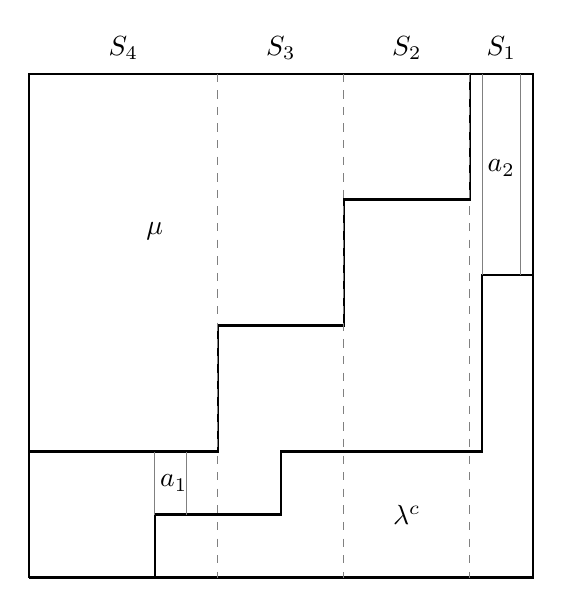
\begin{tikzpicture}[scale = 1.6]
 \draw[black, thick] (0,0) -- (4,0) -- (4,4) -- (0,4) -- (0,0);
 \draw[black, thick] (0,1) -- (1.5,1) -- (1.5,2) -- (2.5,2) -- (2.5,3) -- (3.5,3) -- (3.5,4);
 \draw (1,2.75) node{$\mu$};
 \draw[gray, dashed] (1.5,4) -- (1.5,0);
 \draw[gray, dashed] (2.5,4) -- (2.5,0);
 \draw[gray, dashed] (3.5,4) -- (3.5,0);
 \draw[black, thick] (1,0) -- (1,0.5) -- (2,0.5) -- (2,1) -- (3.6,1) -- (3.6,2.4) -- (4,2.4);
 \draw (1.15,0.75) node{$a_1$};
 \draw[very thin, gray] (1,0.5)--(1,1);
 \draw[very thin, gray] (1.25,0.5)--(1.25,1);
 \draw (3.75, 3.25) node{$a_2$};
 \draw[very thin, gray] (3.6,2.4)--(3.6,4);
 \draw[very thin, gray] (3.9,2.4)--(3.9,4);
 \draw (3,0.5) node{$\lambda^c$};
 \draw (0.75,4.2) node{$S_4$};
 \draw (2,4.2) node{$S_3$};
 \draw (3,4.2) node{$S_2$};
 \draw (3.75,4.2) node{$S_1$};
 
 
 \end{tikzpicture}
%\end{center}
 \caption{}
 \label{Case1}
\end{figure}

\begin{proof}
 Since $\mu$ and $\lambda^\vee$ are not rectangles, $p\geq 3$ and $q\geq 2$. For $1\leq i\leq q+1$, set $S_i = \{\mu_i+1,\dots, \mu_{i-1}\}$, where $\mu_0 = \lambda_1$ and $\mu_{q+1} = 0$.

 By construction, 
 \begin{equation}
 \label{eq:samestart}
 U(c) = U(d)\text{ for }c, d \in S_i
 \end{equation}
 and
 \begin{equation}
 \label{eq:greaterstart}
 U(c) < U(d)\text{ for }c \in S_i, d \in S_j\text{ with }i > j.
 \end{equation}
 
 Denote
 \begin{equation}
 a_1 = \min\{k: L(k) < \ell(\lambda)\} \text{ and } a_2 = \min\{k:L(k) = l_1\}.
 \end{equation}
 Note that by construction $L(1)>L(a_1)>L(a_2)=L(\lambda_1)$, so in particular $1<a_1<a_2$. If $a_1\not\in S_1\cup S_{q+1}$, then columns 1, $a_1$ and $\lambda_1$ satisfy Lemma~\ref{lem:nonrect}~\ref{lemma3.4_1}. 
 
 If $a_1 \in S_1$, then $a_1 < a_2$ implies $a_2 \in S_1$. Set $c_1 = a_1,c_2 = a_2$, and $c_3 = \max(S_2), c_4 = \max(S_3)$. Notice that $U(c_1)=U(c_2)$ by~\eqref{eq:samestart}, with $U(c_1),U(c_3),U(c_4)$ all distinct by~\eqref{eq:greaterstart}. Since $c_1$ is the minimum index such that $L(c_1)<\ell(\lambda)$ and $c_1 \in S_1$, we have $L(c_3) = L(c_4) = \ell(\lambda)$. Finally, $L(c_1)=\ell(\lambda)-l_p,L(c_2)=l_1,L(c_3)=\ell(\lambda)$ are all distinct. Thus these four columns satisfy Lemma~\ref{lem:nonrect}~\ref{lemma3.4_2}. 
 
 If $a_1 \in S_{q+1}$ and $a_2 \leq \min(S_{q})$, then let $c_1 = 1$, $c_2 =a_1$, $c_3 = \min(S_{q})$, and $c_4 = \lambda_1$. Then $U(c_1) = U(c_2)$ by~\eqref{eq:samestart}, and $U(c_1),U(c_3),U(c_4)$ are all distinct by~\eqref{eq:greaterstart}. Since $a_2 = \min\{k:L(k) = l_1\}$ and $a_2 \leq c_3$, then $L(c_3) = L(c_4) = l_1$. Furthermore, $L(c_1) = \lambda_1$, $L(c_2)=\ell(\lambda)-l_p$, and $L(c_3) =l_1$ are all distinct. Hence $c_1,c_2,c_3,$ and $c_4$ satisfy Lemma~\ref{lem:nonrect}~\ref{lemma3.4_2}.

 If $a_1 \in S_{q+1}$ and $a_2 > \min(S_{q})$, then columns 1, $\min(S_{q})$, and $\lambda_1$ satisfy Lemma~\ref{lem:nonrect}~\ref{lemma3.4_1}. Since we have exhausted all possibilities for $a_1$ and $a_2$, we conclude that either Lemma~\ref{lem:nonrect}~\ref{lemma3.4_1} or~\ref{lemma3.4_2} always hold.
\end{proof}

\begin{prop}
\label{prop:3col}
If there exist columns $c_1,c_2,c_3$ in $\lambda/\mu$ such that $U(c_1),U(c_2),U(c_3)$ are all distinct and $L(c_1),L(c_2),L(c_3)$ are all distinct, then $s_{\lambda/\mu}(x_1,\ldots,x_{\rho+1})$ is not multiplicity-free.
\end{prop}
\begin{proof}


First consider the case where $\lambda/\mu$ consists of only those three columns, and without loss of generality say that $c_1=3$, $c_2=2$, and $c_3=1$. Let $\rho_i \coloneqq \CS _{c_i}(\lambda/\mu)$ for $i \in \{1,2,3\}$.

Our goal is to construct two distinct ballot fillings of $\lambda/\mu$ with the same content. In both fillings, we fill column $c_1$ with the numbers from $1$ to $\rho_1$. The entries of column $c_2$ and column $c_3$ will depend on the relative sizes of $\rho_1$, $\rho_2$, and $\rho_3$:


\begin{Case}
%\noindent \emph
{\hypertargeta{prop3.5case_1}{Case 1} $(\rho_1\leq \rho_2 < \rho_3)$} 
For Filling 1, fill column $c_2$ with $[\rho_2]$ and column $c_3$ with $[\rho_3+1]\setminus \{\rho_1\}$. For Filling 2, fill column $c_2$ with $[\rho_2+1]\setminus \{\rho_1\}$ and column $c_3$ with $[\rho_3+1]\setminus \{\rho_2+1\}$.
\end{Case}

\begin{Case}
%\noindent \emph
{\hypertargeta{prop3.5case_2}{Case 2} $(\rho_1< \rho_3 \leq \rho_2)$} 
For Filling 1, fill column $c_2$ with $[\rho_2]$ and column $c_3$ with $([\rho_3]\setminus \{\rho_1\})\cup \{\rho_2+1\}$. For Filling 2, fill column $c_2$ with $[\rho_2+1]\setminus \{\rho_1\}$ and column $c_3$ with $[ \rho_3]$.
\end{Case}

\begin{Case}
%\noindent \emph
{\hypertargeta{prop3.5case_3}{Case 3} $(\rho_2\leq \rho_1 < \rho_3)$} 
For Filling 1, fill column $c_2$ with $[\rho_2]$ and column $c_3$ with $[\rho_3+1]\setminus \{\rho_2\}$. For Filling 2, fill column $c_2$ with $[\rho_2-1]\cup\{\rho_1+1\}$ and column $c_3$ with $[\rho_3+1]\setminus\{\rho_1+1\}$.
\end{Case}

\begin{Case}
%\noindent \emph
{\hypertargeta{prop3.5case_4}{Case 4} $(\rho_2< \rho_3 \leq \rho_1)$} For Filling 1, fill column $c_2$ with $[\rho_2]$ and column $c_3$ with $([\rho_3]\setminus \{\rho_2\})\cup \{\rho_1+1\}$. For Filling 2, fill column $c_2$ with $[\rho_2-1]\cup\{\rho_1+1\}$ and column $c_3$ with $[\rho_3]$.
\end{Case}

\begin{Case}
%\noindent \emph
{\hypertargeta{prop3.5case_5}{Case 5} $(\rho_3\leq \rho_1 \leq \rho_2)$} 
For Filling 1, fill column $c_2$ with $[\rho_2]$ and column $c_3$ with $[\rho_3-1]\cup \{ \rho_2+1\}$. For Filling 2, fill column $c_2$ with $[\rho_2+1]\setminus \{\rho_1\}$ and column $c_3$ with $[\rho_3-1]\cup \{\rho_1\}$.
\end{Case}

\begin{Case}
%\noindent \emph
{\hypertargeta{prop3.5case_6}{Case 6} $(\rho_3\leq \rho_2 \leq \rho_1)$} 
For Filling 1, fill column $c_2$ with $[\rho_2]$ and column $c_3$ with $[\rho_3-1]\cup \{\rho_1+1\}$. For Filling 2, fill column $c_2$ with $[\rho_2-1]\cup \{\rho_1+1\}$ and column $c_3$ with $[\rho_3-1]\cup\{ \rho_2\}$.
\end{Case}


In all of the above cases, both fillings have the same content, and they are strictly increasing within columns. Similarly, in all cases the column reading word is ballot. It remains to show that the fillings are weakly increasing within rows.


\begin{claim}
\label{claim:c2c3}
Let $T$ be any one of the fillings defined in the six cases above. 
\begin{enumerate}[label=(\Roman{*})]
\item\label{claim3.6_1} If $(r,c_2),(r,c_3)\in \lambda/\mu$, then $T(r,c_3) \leq T(r,c_2)$.
\item\label{claim3.6_2} If $(r,c_1),(r,c_2)\in \lambda/\mu$, then $T(r,c_2) \leq T(r,c_1)$.
\end{enumerate}
\end{claim}
\begin{proof}
We first prove~\ref{claim3.6_1}. Since $U(c_3)>U(c_2)$, at most the top $\rho_2-1$ boxes of column $c_3$ are to the left of a box in column $c_2$. In addition, there is at least one box in column $c_2$ in a higher row than the highest box in column $c_3$. Similarly, because $L(c_3)>L(c_2)$, at most the top $\rho_3-1$ labels of $c_3$ are to the left of a label of column $c_2$.

Combining these two facts, we know that at most the top $\min(\rho_2,\rho_3)-1$ boxes in column $c_3$ have a box in column $c_2$ directly to the right. Notice that in all of the cases of the fillings above, for $1\leq k\leq \min(\rho_2,\rho_3)-1$, the $k^{th}$ box from the top of column $c_3$ has a value of at most $k+1$, and its right neighbor is at least the $(k+1)^{th}$ box from the top of column $c_2$. Thus even if column $c_2$ was minimally filled, its entries would still be larger than the corresponding entries in column $c_3$, which proves the claim.

The proof of~\ref{claim3.6_2} follows by the same logic as the proof of~\ref{claim3.6_1}.
\end{proof}

This completes the proof in the case where $\lambda/\mu$ consists of exactly three columns. If $\lambda/\mu$ has more than three columns, then let $\lambda^*/\mu^*$ be the skew shape consisting of only the three columns indexed by $c_1$, $c_2$, and $c_3$ in the statement of the theorem. By Corollary~\ref{Cor:GUT2}, $s_{\lambda^*/\mu^*}(x_1,\dots, x_{\rho(\lambda^*/\mu^*) + 1})$ is not multiplicity-free implies $s_{\lambda/\mu}(x_1,\dots, x_{\rho(\lambda/\mu) + 1})$ is not multiplicity-free.
\end{proof}

